\chapter{Plasmonic Nanomaterials}\label{sec:background:Plasmonics}

\section{Introduction}
\begin{itemize}
    \item The response of a metal surface to incident light can be modelled in terms of plasma oscillations. By treating the metal as a free-electron gas (plasma) surrounding a lattice of positive charges, the electromagnetic response can be described by the motion of this plasma in response to external electromagnetic fields
    \item At a metal-dielectric interface, surface plasmon polaritons describe the coupling of incident light to induced propagating electron density waves on the metal surface. These coupled waves are known as surface plasmon polaritons (SPPs).
    \item SPPs propagate along the metal-dielectric interface, with an exponentially decaying intensity normal to the surface.
    \item We consider an interface between a metal and a dielectric, of permitivities $\varepsilon_1$ and $\varepsilon_2$ respectively. The metal requires that ${\mathop{\rm Re}\nolimits}(\varepsilon_1)<0$ (figure~\ref{fig:background:Plasmonics:SPP}a).
    \item In this configuration, the dispersion relation for a surface plasmon polariton propagating in the $x$ direction, oscillating at frequency $\omega$, is given by equation~\ref{eq:Plasmonics:SPPdispersion}.
    \item Conservation of momentum must be considered when optically exciting surface plasmon polaritons.
    \begin{itemize}
        \item For light incident on the interface via the dielectric described by $\varepsilon_2$, the optical dispersion relation $k_0 = \omega / c = \omega \sqrt{\mu_0 \varepsilon_2}$ shows that the projection of the optical momentum in the direction of SPP propagation will always be lower than that of the SPP (figure~\ref{fig:background:Plasmonics:SPP}b).
        \item Various experimental configurations have been dmeonstrated to allow the excitation of SPPs with optical radiation. These commonly involve exciting a SPP at a metal-dielectric interface with light propagating through a different dielectric, interacting at an adjascent interface.
        \item Examples of Kretschmann and Otto geometries
    \end{itemize}
\end{itemize}

\begin{equation}\label{eq:Plasmonics:SPPdispersion}
    k^{SPP}_{x} = k_0 \sqrt{\frac{\varepsilon_{1}\varepsilon_{2}}{\varepsilon_{1}+\varepsilon_{2}}} = \frac{\omega}{c} \sqrt{\frac{\varepsilon_{1}\varepsilon_{2}}{\varepsilon_{1}+\varepsilon_{2}}}
\end{equation}

\begin{figure}[htb!]
    \centering
    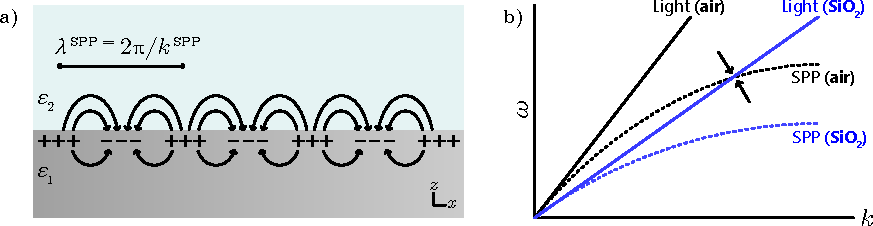
\includegraphics[scale=1.0]{./figures/background/plasmonics/spp.pdf}
    \caption{\label{fig:background:Plasmonics:SPP} WRITE CAPTION \textbf{a)} Surface plasmon polariton at a metal-dielectric interface. \textbf{b)} Schematic of SPP dispersion relations. For any particular interface, SPPs cannot be excited by light impinging from the dielectric at that interface. Light propagating through glass can however be phase-matched to a SPP at a metal-air interface, for example. }
\end{figure}


\section{Localised Surface Plasmons}\label{sec:background:Plasmonics:Metamaterials}
\begin{itemize}
    \item For small diameter $d \ll \lambda$ metallic nanoparticles, the phase of the driving electromagnetic field can be assumed constant over the particle (the ``quasi-static approximation'').
    \item In this lowest-order approximation, the electron gas is driven to coherently oscillate at the particle surface. The response of this particle to incident light can thus be described by an induced dipole moment $\bf{\tilde p}$, much like the simple Lorentz oscilaltor in section~\ref{sec:background:NonlinearOptics:lorentz} (figure~\ref{fig:background:Plasmonics:LSP}a).
    \item For a metallic nanoparticle of permittivity $\varepsilon_1$ surrounded by a dielectric of permittivity $\varepsilon_2$, the induced dipole moment is described by equation~\ref{eq:Plasmonics:LSPdipole}. Here, ${\tilde \alpha }$ describes the complex polarizability of the particle, and depends strongly on the nanoparticle material, geometry, and the permittivity of the surrounding medium.
    \item Importantly, the induced oscillating dipole is non-propagating, and so the momentum-matching requirements for exciting propagating surface plasmon polaritons are alleviated. The localised surface plasmon can be driven coherently by any incident light, and will reach a maximum excitation efficiency at a particular resonant frequency determined by the effective polarizability ${\tilde \alpha }(\omega)$.
    \item Analytical expressions for ${\tilde \alpha }(\omega)$ are well established for simple spherical nanoparticles of radius $a$ and permittivity $\varepsilon(\omega)$ [REFS], given by equation~\ref{eq:Plasmonics:LSPalphaSphere}. At the point where $\varepsilon (\omega) + 2\varepsilon_2 (\omega)$ is at it's minimum, the polarizability is maximally enhanced, determining the resonant frequency of the localised surface plasmon.
    \item However, in many systems the nanoparticle geometry is significantly more complex, and the LSP resonance cannot be determined analytically
\end{itemize}

\begin{equation}\label{eq:Plasmonics:LSPdipole}
    {\bf{\tilde p}} = {{\tilde \alpha }}{\bf{\tilde E}}
\end{equation}
\begin{equation}\label{eq:Plasmonics:LSPalphaSphere}
    {\tilde \alpha } = 4\pi a^3 \frac{\varepsilon (\omega) - \varepsilon_2 (\omega)}{\varepsilon (\omega) + 2\varepsilon_2 (\omega)}
\end{equation}

\subsection{Metamaterials and Effective Media}
\begin{itemize}
    \item In cases of arrays of nanoparticles exhibiting LSPs, the system can be modelled as an array of oscillators, with effective polarizabilities. The macroscopic behaviour of the array can then be described as an effective medium, with a susceptibility describing its optical response as in section~\ref{sec:background:NonlinearOptics:susceptibility}
\end{itemize}

\begin{figure}[htb!]
    \centering
    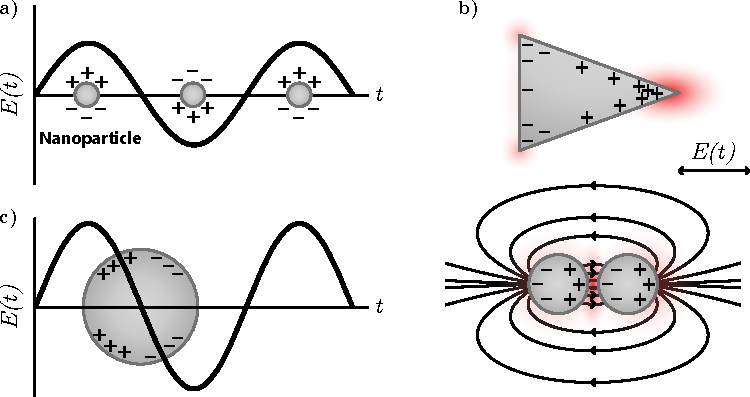
\includegraphics[scale=1.0]{./figures/background/plasmonics/lsp.pdf}
    \caption{\label{fig:background:Plasmonics:LSP} WRITE CAPTION \textbf{a)} For sub-wavelength metallic nanoparticles, charge is coherently driven at the surface, and the particle can be approximated to an oscillating dipole. \textbf{b)} A pair of nanoparticles separated by some small distance will couple via the near-field, and function as a single dipole with an additional capacitance from the gap. Charge is efficiently confined to the inner surface, resulting in an enhanced electric field intensity between the two particles.}
\end{figure}


\section{Electromagnetic Field Confinement}\label{sec:Plasmonics:confinement}
\begin{itemize}
    \item Enhancement via localised surface plasmon resonance (excitation/scattering). 
    \begin{itemize}
        \item When a metallic nanoparticle is excited close to a plasmon resonance, the induced dipole oscillates at maximum amplitude. This results in a resonant scattering and absorption of light, leading to locally enhanced electromagnetic fields around the particle. For sub-wavelength nanoparticles, this allows some degree of sub-wavelength field confinement, since the near-field response is dependent on the particle geometry.
        \item Example of enhancement from single nanoparticles
    \end{itemize}
    \item Enhancement via coupled localised surface plasmons (capacitance)
        \begin{itemize}
            \item A simple example is a pair of sub-wavelength nanoparticles, separated by a distance $d \ll \lambda$. This system behaves as a pair of point dipoles interacting via the near-field (figure~\ref{fig:background:Plasmonics:LSP}b). In the limit of small separation $d$, the coupled system will radiate as a dipole, and resonantly scatter when excited at resonance. However, when driven by a field poalrised along the chain axis, the resonant frequency will be shifted. The gap between particles introduces a capacitance, dependent on particle geometry and separation, which shifts the resonant frequency of the hybridised plasmon mode along that axis.
            \item Crucially, the capacitance of the gap results in the confinement of charge on the inner surfaces of the particles. This confinement of charge directly leads to confinement of the electromagnetic fields in the region between particles.
            \item Example of enhancement from coupled nanoparticles
        \end{itemize}
    \item Enhancement via lightning-rod effect (charge confinement)
    \begin{itemize}
        \item An additional enhancement in field confinement can come from the ``lightning-rod effect''. In the context of electrostatics, the ligtning-rod effect describes the confinement of electric fields at sharp gradients of metallic structures, such as corners or tapered tips. Charge is confined more efficiently to regions of sharp surface gradients on a charged conductor, and so the electric field lines at the surface of the conductor will be localised around these sharp features.
        \item While not necesarily a relevant enhancement when considering coupled spherical nanoparticles, nanostructure geometries with sharper features, especially when multiple sharp features are closely coupled to eachother, can greatly benefit from the additional confinement associated with the lightning-rod effect.
        \item Examples of field hotspots at the edges of nanostructures
        \begin{itemize}
            \item Direct observation of near-field localisation around the sharp features of a chiral nanostructure by ``nano-jets''~\cite{Valev2012d}
        \end{itemize}
    \end{itemize}
    
    \item Applications (literature review)
    \begin{itemize}
        \item Frequently used for SERS
        \item Sub-wavelength imaging (brief)
        \item Enhancement in chiral-optical measurements. Anything NOT about superchiral light, eg molecules between coupled spherical nanoparticles (see review sections).
        \item Enhanced nonlinear effects (due to strong intensity dependence) (most relevant to this work)
    \end{itemize}
\end{itemize}

\section{Beyond the Quasi-Static Approximation}
\begin{itemize}
    \item Intermediate regieme of nanostructures, beyond the quasi-static approximation. Structure dimensions are close to, or larger than, the wavelength.
    \item The near-field optical behaviour in this regieme can be understood in terms of higher order current density modes.
    \begin{itemize}
        \item The geometry of the metallic surface will permit a set of plasmon modes.
        \item Higher order plasmon modes can be excited across the surface of the structure.
        \item These modes are non-propagating standing waves, and have zero net momentum. Thus, even in this intermediate regieme momentum matching is not a requirement to excite surface plasmons.
    \end{itemize}
    \item Literature review
    \begin{itemize}
        \item Zheng's work demonstrated that the plasmonic response of metallic nanostructures in this intermediate regieme can be decomposed into a set of current density eigenmodes~\cite{Zheng2012}. This work was extended to collections of coupled nanostructures~\cite{Zheng2013}. 
        \item The optical response can be further understood by applying group theory to the plasmonic eigenmode set~\cite{Zheng2015}, allowing the current density modes to be grouped by the optical polarisation states that exclusively excite them.
    \end{itemize}
\end{itemize}


\section{Chiral Plasmonic Nanostructures}
\begin{itemize}
    \item Freedom of fabrication techniques allow symmetries to be explored.
    \item Second-order nonlinear processes, which already enhance chiroptical measurements, can themselves be enhanced as described in section~\ref{sec:Plasmonics:confinement}.
    \item Literature review
\end{itemize}

\subsection{Superchiral Fields from Plasmonic Metasurfaces}
\begin{itemize}
    \item Literature review (from \cite{Collins2017})
\end{itemize}